\clearpage
\section{Local Line Following: One Program on Pi}
\label{app:line-follower}
\label{sec:local-controller}

This section describes the local controller implemented by \texttt{lineFolower\_ver1.py}, with defaults updated on September 24, 2026. It uses the three-channel calibration from Appendix~\ref{app:photo3-calibration} and independently drives the left and right wheels. The controller permits an inside wheel to reverse on a sharp curve. Its three decisions are: whether any sensor detects tape, whether a channel has changed enough to update its accepted reading, and whether a left or right gradient is distinguishable from zero. One parameter, $k=\texttt{nSigma}$, controls all three decisions; the default is $k=2.5$.


\subsection{Execution and Data Flow}
The actual source filename is \texttt{lineFolower\_ver1.py} (not \texttt{lineFolower\_v1.py}), under \path{/home/pi/robot0/}. The master source is on Pi; the Mac's \texttt{robot0} tree is a mirror. The program imports serial helpers from \texttt{photo3\_calib.py}; the existing local program is not a standalone one-file distribution.

Before opening UART, it validates the calibration and arguments. It then opens \texttt{/dev/serial0} exclusively at 115200 baud, verifies firmware features and pin mapping, requests \texttt{STOPALL}, and checks stopped status and an ADC triplet. The normal loop is sequential: request \texttt{ADC3}, evaluate the following equations, send \texttt{MOTORS left right} or \texttt{STOPALL}, require an acknowledgement, and sleep for the remainder of the target period. Desktop and ASUS are used for SSH and management; neither computes steering in this mode.

\begin{figure}[H]
\centering
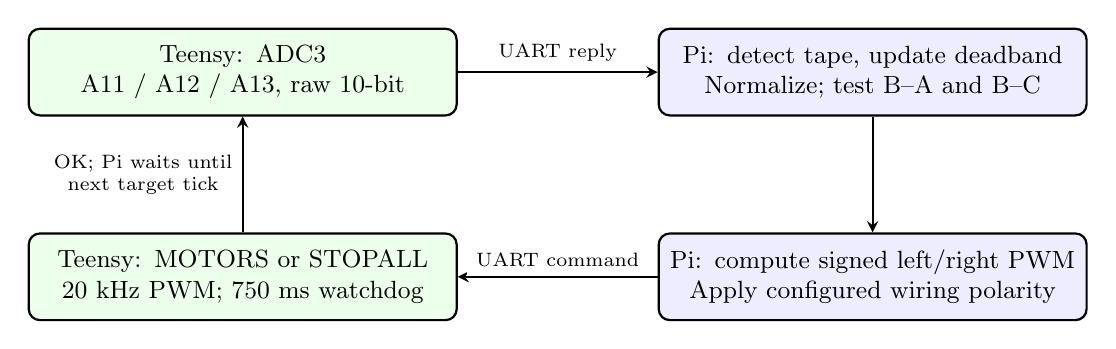
\begin{tikzpicture}[font=\small,>=stealth,
 block/.style={draw,thick,rounded corners,align=center,text width=5.2cm,minimum height=1.1cm},
 flowarrow/.style={->,thick},note/.style={font=\scriptsize,fill=white,align=center}]
\node[block,fill=green!8] (adc) at (0,0) {Teensy: ADC3\\A11 / A12 / A13, raw 10-bit};
\node[block,fill=blue!7] (interpret) at (8,0) {Pi: detect tape, update deadband\\Normalize; test B--A and B--C};
\node[block,fill=blue!7] (decide) at (8,-2.6) {Pi: compute signed left/right PWM\\Apply configured wiring polarity};
\node[block,fill=green!8] (motor) at (0,-2.6) {Teensy: MOTORS or STOPALL\\20 kHz PWM; 750 ms watchdog};
\draw[flowarrow] (adc) -- node[note,above] {UART reply} (interpret);
\draw[flowarrow] (interpret) -- (decide);
\draw[flowarrow] (decide) -- node[note,above] {UART command} (motor);
\draw[flowarrow] (motor) -- node[note,left] {OK; Pi waits until\\next target tick} (adc);
\end{tikzpicture}

\caption{Implemented local controller. All line-following decisions run on Pi; Teensy supplies ADC acquisition and hardware PWM. Three ADC channels are read sequentially.}
\label{fig:local-controller}
\end{figure}

The default period is 50\,ms (20\,Hz), configurable from 10 to 100\,Hz. This is a target, not a hard real-time guarantee: each serial read/write has a 150\,ms timeout and the loop waits for replies. Console status is limited to about 5\,Hz. The current firmware source configures both wheel PWM channels at 20\,kHz, independently of the Python update rate. A PWM command is not a measured wheel speed.

\subsection{Normalization and Tape Detection}
Let $a_i(t)$ be the current raw ADC value of sensor $i$, and let its white and black calibration means be $\mu_{i,W}$ and $\mu_{i,B}$. Define $\Delta_i=\mu_{i,B}-\mu_{i,W}>0$ and
\begin{equation}
x_i(a)=\operatorname{clip}_{[0,1]}\!\left(\frac{a-\mu_{i,W}}{\Delta_i}\right).
\label{eq:lf-normalize}
\end{equation}
Thus white maps to zero, black to one, and each channel's pedestal and gain are accounted for separately. Clipping limits the controller input when a reading is outside its calibrated endpoint means.

Tape is considered present if at least one \emph{current raw} reading exceeds its white mean by more than $k$ white standard deviations:
\begin{equation}
\mathrm{tape}(t)=\bigvee_{i\in\{A,B,C\}}
\left[a_i(t)>\mu_{i,W}+k\sigma_{i,W}\right].
\label{eq:lf-tape}
\end{equation}
If no channel passes this test, both motors stop and the robot waits for manual repositioning. Sampling continues, and following resumes when a channel passes again, provided the run time has not expired. Detection uses the spread of readings on white.

\subsection{Significance of a Change in One Channel}
Let $\widehat a_i$ denote the last accepted ADC reading. To estimate noise between the measured white and black endpoints, use the linear interpolation
\begin{equation}
s_i(a)=\bigl[1-x_i(a)\bigr]\sigma_{i,W}+x_i(a)\sigma_{i,B}.
\label{eq:lf-noise-model}
\end{equation}
This interpolation provides an empirical noise model across the reflectance range. Evaluate it at both the new and accepted readings, and combine their uncertainties in quadrature:
\begin{equation}
s_{i,\mathrm{change}}=
\sqrt{s_i\bigl(a_i(t)\bigr)^2+s_i(\widehat a_i)^2}.
\end{equation}
The accepted reading is updated according to
\begin{equation}
\widehat a_i\leftarrow
\begin{cases}
a_i(t),& |a_i(t)-\widehat a_i|>k\,s_{i,\mathrm{change}},\\
\widehat a_i,& \text{otherwise}.
\end{cases}
\label{eq:lf-update}
\end{equation}
The reference stays at the last accepted value, so gradual drift can eventually exceed the band. Equal single-reading uncertainties $s$ give a difference uncertainty $\sqrt{2}\,s$.

The first triplet is accepted immediately. The accepted values are also reset during tape loss and on resumption, so stale steering cannot prevent stopping or restarting. Equation~\eqref{eq:lf-tape} is evaluated every cycle independently of held steering readings, but still uses the same $k$. Setting $k=0$ accepts every triplet and detects tape whenever a current ADC is strictly above its white mean.

\subsection{Significance of the Steering Gradients}
Normalize the accepted readings as $\widehat x_i=x_i(\widehat a_i)$. The two steering differences are
\begin{equation}
g_L=\widehat x_B-\widehat x_A,\qquad
g_R=\widehat x_B-\widehat x_C.
\label{eq:lf-gradients}
\end{equation}
Their noise must be expressed in the same normalized units. For each channel,
\begin{equation}
\nu_i=\frac{(1-\widehat x_i)\sigma_{i,W}+\widehat x_i\sigma_{i,B}}{\Delta_i},
\qquad
\nu_L=\sqrt{\nu_B^2+\nu_A^2},\quad
\nu_R=\sqrt{\nu_B^2+\nu_C^2}.
\label{eq:lf-gradient-noise}
\end{equation}
Applying the shared nSigma setting gives
\begin{equation}
\widetilde g_j=
\begin{cases}
g_j,& |g_j|>k\nu_j,\\
0,& |g_j|\le k\nu_j,
\end{cases}
\qquad j\in\{L,R\}.
\label{eq:lf-gradient-gate}
\end{equation}
Both positive and negative gradients are tested. A statistically insignificant gradient contributes zero to steering, leaving the wheel at its base forward command. For example, normalized channel deviations $\nu_A=0.03$ and $\nu_B=0.04$ give $\nu_L=0.05$. At $k=2.5$, $|g_L|$ must exceed 0.125: a difference of 0.10 is suppressed, whereas 0.20 is retained.

The quadrature formulas treat the reading errors as independent and use the calibrated endpoint means as fixed references. Under this empirical noise model, $k$ is a practical significance multiplier. The same $k$ has three roles: raising it requires more contrast above white, larger temporal changes, and stronger spatial gradients.

\subsection{Wheel Commands and Resulting Motion}
When tape is present, the significant gradients determine the physical-direction PWM commands:
\begin{align}
D&=\operatorname{round}(255s),\\
p_L&=\operatorname{round}\!\left[D\operatorname{clip}_{[-1,1]}(0.5+\widetilde g_L)\right],\\
p_R&=\operatorname{round}\!\left[D\operatorname{clip}_{[-1,1]}(0.5+\widetilde g_R)\right],
\label{eq:lf-wheel-law}
\end{align}
where $s=\texttt{speed}$, default 0.5. Positive commands mean forward and negative commands mean reverse. Fixed wiring signs are applied only when transmitting these commands. With the current \texttt{rr} polarity, both transmitted signs are reversed relative to physical forward.

The offset 0.5 maintains forward drive when a gradient is zero or suppressed. For a significant gradient, the associated wheel stops at $g=-0.5$ and reverses below that value. Because $g\in[-1,1]$, the command factor spans $[-0.5,1]$ after clipping. At the default $s=0.5$, the nominal command range is approximately $-0.25$ to $+0.5$, with 8-bit rounding.

When A rises relative to B, the \emph{left} wheel slows and can reverse, turning toward that side. When C rises relative to B, the \emph{right} wheel does so. If all sensors lose tape according to Eq.~\eqref{eq:lf-tape}, both commands are replaced by a motor stop regardless of gradient significance. The displayed values $p_L/255$ and $p_R/255$ are commanded PWM fractions; small nonzero values may be insufficient to start a loaded motor.

\subsection{Representative Responses and Operating Parameters}
Table~\ref{tab:lf-responses} illustrates the wheel law before integer rounding. Nonzero gradients in its first five rows are assumed to pass Eq.~\eqref{eq:lf-gradient-gate}, and tape must pass Eq.~\eqref{eq:lf-tape}.
\begin{table}[H]
\centering\small
\caption{Idealized line-following responses. Wheel factors multiply base PWM $D$.}
\label{tab:lf-responses}
\begin{tabular}{@{}L{4.0cm}L{2.4cm}L{2.4cm}L{7.3cm}@{}}
\toprule
\textbf{Accepted A, B, C} & \textbf{Left factor} & \textbf{Right factor} & \textbf{Robot action} \\
\midrule
0, 1, 0 & 1 & 1 & Centered tape: equal forward commands. \\
1, 1, 0 & 0.5 & 1 & Left wheel slows; curve left. \\
0, 1, 1 & 1 & 0.5 & Right wheel slows; curve right. \\
1, 0, 0 & $-0.5$ & 0.5 & Left wheel reverses; turn left in place ideally. \\
0, 0, 1 & 0.5 & $-0.5$ & Right wheel reverses; turn right in place ideally. \\
Both gradients insignificant & 0.5 & 0.5 & Equal forward commands while tape is detected. \\
No current channel detects tape & 0 & 0 & Stop and wait for repositioning. \\
\bottomrule
\end{tabular}
\end{table}

The controller targets 20 updates per second and prints current ADCs, accepted normalized readings and commanded wheel fractions at about 5\,Hz. Commands continue to refresh while steering readings are held. A run ends after 60\,s by default; stopped waiting is included in this limit, which starts after initial verification. Communication latency limits exact stopping time. Time expiry, interruption or communication failure requests a stop; the motor firmware also has a 750\,ms drive-command watchdog. These stops put the driver in standby, allowing the wheels to coast to rest.

\begin{table}[H]
\centering\small
\caption{Line-follower parameters. All effective values are printed at startup.}
\label{tab:lf-parameters}
\begin{tabular}{@{}L{3.4cm}L{3.2cm}L{9.5cm}@{}}
\toprule
\textbf{Parameter} & \textbf{Default} & \textbf{Meaning} \\
\midrule
\texttt{-t}, \texttt{--time} & 60\,s & Maximum control-loop duration, including stopped waiting; positive. \\
\texttt{--speed} & 0.5 & Base PWM scale $s$; $0\le s\le1$. \\
\texttt{--nSigma} & 2.5 & Nonnegative multiplier $k$ in tape detection, reading updates and gradient tests. \\
\texttt{--rate} & 20\,Hz & Target control-loop rate; 10--100\,Hz. \\
\texttt{--polarity} & From calibration & Left/right wiring signs, currently \texttt{rr}; options \texttt{ff}, \texttt{fr}, \texttt{rf}, \texttt{rr}. \\
\texttt{--calibration} & Latest JSON & \path{out/photo3_calib.latest.json}, relative to the program location; requires complete, valid calibration. \\
\texttt{--port} & \texttt{/dev/serial0} & Pi--Teensy UART device. \\
\texttt{--check} & False & Verify calibration and readout while keeping motors stopped. \\
\bottomrule
\end{tabular}
\end{table}
